%\documentclass[twocolumn,showpacs,preprintnumbers,amsmath,amssymb, floatfix]{revtex4}
\documentclass[aps,prb,preprint,preprintnumbers,amsmath,amssymb,floatfix,superscriptaddress]{revtex4}
%\documentclass[aps,prb,twocolumn,superscriptaddress,preprintnumbers,amsmath,amssymb,floatfix]{revtex4}

\usepackage{graphicx}
\usepackage{epstopdf}
\usepackage{ifthen}
\usepackage{dcolumn}
\usepackage{bm}
\usepackage{multirow}
\usepackage{booktabs}
\usepackage{amsbsy}
\usepackage{amsmath}
\usepackage{amssymb}
\usepackage{subfigure}
\usepackage{booktabs}
\usepackage{verbatim}
\usepackage{hyperref}

\graphicspath{
{/Users/mullspace/Dropbox/git/plots.nogit/images/}
{/home/schuberm/Dropbox/git/plots.nogit/images/}
{/home/mull/Dropbox/git/plots.nogit/images/}
{/home/mullspace/Dropbox/git/plots.nogit/images/}
}

%--------------------------------------------------------------------------
%DEFINE COMMANDS
%--------------------------------------------------------------------------
\newcommand{\EXP}[1]{\exp\mspace{-5.0mu}\left[#1\right]\mspace{-3.0mu}}

\newcommand{\SUM}[2]{\ifthenelse{\equal{#1}{0}}{\sum_{
\alpha_{#2},b_{#2},l_{#2}}^{3,4L,N}} {\ifthenelse{\equal{#1}{1}}{\sum_{
\alpha_{#2},b_{#2}}^{3,n}}{\sum_{\pmb{\kappa}#2,\nu#2}^{N,3n}}}}

\newcommand{\ab}[2]{\mspace{-4.0mu}\left(\mspace{-8.0mu}
\begin{smallmatrix}&\ifthenelse{\equal{#1}{}}{a}{#1} \\&\ifthenelse
{\equal{#2}{}}{b}{#2}\end{smallmatrix}\mspace{-3.0mu}\right)}

\newcommand{\kvba}{\mspace{-4.0mu}\left(\mspace{-8.0mu}
\begin{smallmatrix} &\pmb{\kappa} &b \\ &\nu &\alpha\end{smallmatrix}
\mspace{-3.0mu}\right)}

\newcommand{\kvbap}{\mspace{-4.0mu}\left(\mspace{-8.0mu}
\begin{smallmatrix} &\pmb{\kappa}' &b \\ &\nu' &\alpha\end{smallmatrix}
\mspace{-3.0mu}\right)}

\newcommand{\kvt}{\mspace{-4.0mu}\left(\mspace{-8.0mu}
\begin{smallmatrix}&\pmb{\kappa} \\&\nu\end{smallmatrix}
\mspace{-2.0mu},t\right)}

\newcommand{\kvw}{\mspace{-4.0mu}\left(\mspace{-8.0mu}
\begin{smallmatrix}&\pmb{\kappa} \\&\nu\end{smallmatrix}
\mspace{-2.0mu},\omega\right)}

\newcommand{\kv}{\mspace{-4.0mu}\left(\mspace{-8.0mu}
\begin{smallmatrix}&\pmb{\kappa} \\&\nu\end{smallmatrix}
\mspace{-3.0mu}\right)}

\newcommand{\kvp}{\mspace{-4.0mu}\left(\mspace{-8.0mu}
\begin{smallmatrix}&\pmb{\kappa'} \\&\nu'\end{smallmatrix}
\mspace{-3.0mu}\right)}

\newcommand{\kw}{\mspace{-4.0mu}\left(\mspace{-8.0mu}
\begin{smallmatrix}&\pmb{\kappa} \\&\omega\end{smallmatrix}
\mspace{-3.0mu}\right)}

\newcommand{\lbt}{\mspace{-4.0mu}\left(\mspace{-8.0mu}
\begin{smallmatrix}&l \\&b\end{smallmatrix}\mspace{-2.0mu},t\right)}
%--------------------------------------------------------------------------
%END COMMANDS
%--------------------------------------------------------------------------
%--------------------------------------------------------------------------
\begin{document}

\title{Disruption of Superlattice Phonons by Interfacial Mixing}
\author{Samuel C. Huberman}
\affiliation{Department of Mechanical \& Industrial Engineering, University of Toronto, 
Toronto, Ontario M5S 3G8, Canada}
\author{Jason M. Larkin}
\affiliation{Department of Mechanical Engineering\\Carnegie Mellon University\\Pittsburgh, PA 15213}
\author{Alan J. H. McGaughey}
%\email{mcgaughey@cmu.edu}
\affiliation{Department of Mechanical Engineering\\Carnegie Mellon University\\Pittsburgh, PA 15213}
\author{Cristina H. Amon}
\affiliation{Department of Mechanical \& Industrial Engineering, University of Toronto, 
Toronto, Ontario M5S 3G8, Canada}
\affiliation{Department of Mechanical Engineering\\Carnegie Mellon University\\Pittsburgh, PA 15213}

\date{\today}% It is always \today, today,
             %  but any date may be explicitly specified
\vspace{14mm}
  
\begin{abstract}

We use normal mode decomposition to obtain phonon properties from quasi-harmonic lattice dynamics calculations and classical molecular dynamics simulations in unstrained Lennard-Jones argon superlattices with perfect and mixed interfaces. Debye scaling ($\omega^{-2}$) of phonon lifetimes is found at low frequencies in both perfect and mixed superlattices and Rayleigh scaling ($\omega^{-4}$) for intermediate frequencies in mixed superlattices. We find that mixing reduces a phonon's mean free path and for short-period superlattices, lifetimes below the Ioffe-Regel limit are observed. The relaxation-time approximation of the Boltzmann transport equation is used to predict cross-plane and in-plane thermal conductivity. The assumption of perturbative disorder, where Tamura elastic mass defect scattering theory can be applied, was found to be valid for predicting cross-plane thermal conductivities but not in-plane thermal conductivities in mixed superlattices. 

\end{abstract}
\maketitle
%%%%
\section{Introduction}

Superlattices are nanostructures built from periodic alternating layers of dissimilar materials. They offer potential benefits in thermoelectric energy conversion applications because of the ability to independently tune their thermal conductivities by controlling the period thickness of the layers (i.e., secondary periodicity).\cite{broido1995effect,balandin2003mechanism,kim2006thermal} In reality, the interfaces between layers will contain some disorder (i.e., interfacial mixing), affecting the thermal conductivity. To design a superlattice with a tailored thermal conductivity, a rigorous examination of the interplay between the superlattice period thickness and interfacial mixing is necessary. This need provides the impetus for an analysis to elucidate the effects of the secondary periodicity and interfacial mixing on the properties of individual phonon modes. 

Thermal transport in superlattices has been studied using molecular dynamics (MD) simulations and Boltzmann transport equation (BTE) based methods. Previous MD studies used the equilibrium Green-Kubo(GK) \cite {PhysRevB.85.195302,PhysRevB.77.184302} technique or the non-equilibrium \cite{PhysRevB.79.214307,PhysRevB.72.174302,PhysRevB.79.075316} direct method to predict thermal conductivity. Bottom up works using the BTE relied upon the validity of bulk phonon properties\cite{walkauskas:2579,chen:220} and approximations for the specularity and conductance of the internal interfaces.\cite{PhysRevB.57.14958} While these techniques can predict trends in thermal conductivity (i.e.: effect of period length), the effects of the secondary periodicity and interfacial mixing on phonon properties cannot be directly modeled.

The effect of interfacial mixing on the thermal conductivity (but not on individual modes) of Si/Ge superlattices was demonstrated by Landry and McGaughey. They showed that for perfect Si/Ge superlattices thermal conductivity decreased with increasing period length before leveling out while for superlattices with interfacial mixing, the thermal conductivity (lower than the corresponding perfect case) increased with period length before leveling out. \cite{PhysRevB.79.075316} Savic et al. used Monte Carlo integration to the predict the phonon properties in perfect Si/Ge superlattices (i.e., inclusion of the secondary periodicity \textit{without} interfacial mixing) and noted the difference between theory and experiment. \cite{savic:073113} Recent work by Garg et al. used density functional perturbation theory (DFPT) to examine phonon properties in perfect Si/Ge superlattice structures (i.e., inclusion of the secondary periodicity \textit{without} interfacial mixing). They report a significant discrepancy between theoretically predicted and experimentally measured cross-plane thermal conductivities, which they attributed to the exclusion of mass defect scattering in the DFPT calculation but expected to be important in experimental samples. \cite{doi:10.1021/nl202186y} With this result in mind, Luckyanova et al. \cite{Luckyanova16112012} adopted Tamura elastic mass defect scattering theory \cite{tamura_isotope_1983} to modify the DFPT predicted lifetimes through the Matthiesen rule (i.e., inclusion of the secondary periodicity \textit{and} interfacial mixing).
%Recent work by Garg et al. used Density Functional Perturbation Theory (DFPT) to examine phonon properties in Si/Ge superlattice structures to report a significant discrepancy between theoretically predicted and experimentally measured cross-plane thermal conductivities which was attributed to the exclusion of mass defect scattering in the DFPT calculation but expected to be present in experimental samples. \cite{doi:10.1021/nl202186y} This conclusion was echoed by Savic et al. using a Monte Carlo approach to the BTE for Si/Ge superlattices. \cite{savic:073113} The effect of defects on thermal conductivity was demonstrated by Landry and McGaughey, who showed that for perfect Si/Ge superlattices thermal conductivity decreased with increasing period length before eventually leveling out while for superlattices with interfacial mixing, the thermal conductivity increased with period length before eventually leveling out. \cite{PhysRevB.79.075316} With this in mind, Luckyanova et al. \cite{Luckyanova16112012} adopted Tamura elastic mass defect scattering theory \cite{tamura_isotope_1983} to modify the DFPT predicted lifetimes through the Matthiesen rule.
%Mode-by-mode studies are computationally expensive; limiting Broido et al. to a range of short period lengths ($8\times 8$) for Si/Ge.\cite {PhysRevB.70.081310} For similar reasons, the phonon properties for short period superlattices obtained from DFPT were presumed to hold for larger period superlattices \cite{Luckyanova16112012, doi:10.1021/nl202186y} and the phonon lifetimes of low frequency modes used in the Monte Carlo BTE approach are fitted to a power law. \cite{savic:073113}

In this paper, we reveal the direct relationship between the secondary periodicity and interfacial mixing on phonon properties. MD based normal mode decomposition (NMD) is used to predict the full spectrum of phonon properties in unstrained superlattices with perfect and mixed interfaces. The vibrational modes which emerge by using the phonon dispersion based on the secondary periodicity of the layers are hereafter referred to has superlattice phonons. The rest of the paper is organized as follows. In Section~\ref{SEC:modeling}, the superlattice geometry is defined and the NMD algorithm is reviewed. In Section~\ref{SEC:results}, superlattice phonon dispersion, superlattice phonon lifetimes and thermal conductivities predicted from GK, NMD and Tamura theory are presented. In Section~\ref{SEC:sl_phon}, the results are put in context with the concept of phonon coherence.

%The crucial ingredient is to use the eigenvectors (polarization vectors) of the perfect superlattice to obtain lifetimes for both perfect and mixed superlattices. 

\section{Modeling Framework}\label{SEC:modeling}
\subsection{Superlattice structure and interactions}\label{SEC:sl_struc}
%%%
The superlattices are built by placing atoms on a face-centered cubic lattice, with the two species only differentiated by their masses. The atomic interactions are modeled using the Lennard-Jones (LJ) potential for argon with an energy scale of $1.67\times10^{-21}$ J, a length scale, $\sigma$, of $3.4\times10^{-10}$ m, a mass scale, $m$, of $6.63\times10^{-26}$ kg, and are cutoff and shitfed at a radius of $2.5\sigma$. The lighter species has a mass of $m$ and the heavier species has a mass of $3m$. The temperature of all simulations is 20 K, for which the zero-pressure lattice constant is, $a$, 5.315 $\AA$.\cite{mcgaugheythesis} We present results in  dimensionless LJ units are used unless otherwise noted. 
%($E^*=E/\epsilon$, $T^*=Tk_B/\epsilon$, $\omega^*=\omega\sqrt{\sigma^2m_a/\epsilon}$, $k^*=km^{0.5}_a\sigma^2/(\epsilon^{0.5}k_B)$)

Each superlattice is identified by its unit cell, which consists of $L/2$ conventional four-atom unit cells of each species. The unit cell therefore contains $4L$ atoms. As shown in Fig.~\ref{fig:md_domain}(a), one period of a $4\times4$ superlattice has eight monolayers (four of each species). The Brouillin zone is a rectangular prism with boundaries at $2\pi/(La)$ in the cross-plane direction and $2\pi/a$ in the in-plane directions. We consider $2\times2$, $4\times4$, $8\times8$, and $14\times14$ superlattices.
%%%
\begin{figure}[t!]
\begin{center}
\scalebox{0.5}{ \includegraphics{4p_ai.eps}}
\renewcommand{\figure}{Fig.}
\caption{Atomic representation of a $4\times4$ superlattice for (a) perfect and (b) 80/20 interfacial mixing cases. Orange atoms have mass  $m$ and green atoms have mass $3m$.}
\label{fig:md_domain}
\end{center}
\end{figure}
%%%

Interfacial mixing is introduced to a superlattice by flipping the masses of randomly selected atoms in the monolayers adjacent the interfaces until the desired concentrations are reached.\cite{PhysRevB.79.075316} A $4\times4$ superlattice with 80/20 interfacial mixing (the notation corresponds to the concentration of original/foreign species within the monolayers adjacent to the interface) is shown in Fig.~\ref{fig:md_domain}(b).

\subsection{Thermal conductivity prediction}\label{SEC:methods}

As in some previous superlattice studies, \cite{Luckyanova16112012,doi:10.1021/nl202186y} the phonon Boltzmann Transport Equation (BTE) under the single mode relaxation time approximation,\cite{ziman_electrons_2001} is used to predict the thermal conductivity, $k$, in the $\alpha$-direction from
%%%
\begin{equation}\label{EQ:M:conductivity}
\begin{split}
k_{vib,\mathbf{\alpha}}=&\sum_{\nu,\pmb{\kappa}}^{12L,N} c_{ph}\kv
v^{2}_{g,\mathbf{\alpha}}\kv \tau\kv.
\end{split}
\end{equation}
%%%
Here, $c_{ph}\kv$ is the specific heat, $v_{g,\mathbf{\alpha}}$ is the component of the group velocity in the $\alpha$-direction, and $\tau\kv$ is the lifetime of the phonon mode with wavevector $\pmb{\kappa}$ and polarization branch denoted by $\nu$. The summation is over the total number of polarization branches, $12L$, and the number of unit cells in the simulation, $N$. A quantity of interest for nanostructure design purposes \cite{PhysRevB.87.035437} is the phonon mean free path, $\Lambda\kv$, defined as the average distance travelled between scattering events, \cite{ziman_electrons_2001}
%%%
\begin{equation}\label{EQ:M:phonon_mfp}
\begin{split}
\Lambda\kv &= |\pmb{\mathrm{v}}_{g}\kv | \tau\kv,
\end{split}
\end{equation}
%%%
where $\pmb{\mathrm{v}}_{g}\kv$ is the group velocity vector. To obtain the required inputs for Eqs.~(\ref{EQ:M:conductivity}) and~(\ref{EQ:M:phonon_mfp}) , we follow the NMD procedure outlined by McGaughey and Kaviany\cite{PhysRevB.71.184305}, Turney et al.\cite {PhysRevB.79.064301} and Larkin et al.,\cite{jason_inpress} in which atomic velocities obtained from MD simulation are projected onto the normal mode eigenvectors obtained from harmonic lattice dynamics calculations. The mode-dependent specific heat is set to be $k_\mathrm{B}/V$, where $V$ is the volume of the MD domain and $k_\mathrm{B}$ is the Boltzmann constant, because MD simulations are classical and obey Maxwell-Boltzmann statistics. As temperature increases, anharmonicity of the potential energy causes the specific heat to deviate from $k_\mathrm{B}/V$, but the effect is small for LJ systems at the studied temperature of 20 K.\cite{PhysRevB.71.184305} 

The unit cells for the perfect superlattices, as depicted in Fig.~\ref{fig:md_domain}(a), are used as inputs to the harmonic lattice dynamics (HLD) calculations which are performed using GULP\cite{GULP} to obtain harmonic frequencies, $\omega_H \kv$, and eigenvectors, $ \pmb{\mathrm{e}} \kv$, at the allowed wavevectors, which are specified from
%%%
\begin{equation}\label{EQ:NMD:allowdkpt}
\pmb{\kappa} = \sum_{\alpha=1}^3 \pmb{\mathrm{b}}_{\alpha} \frac{n_{\alpha}}{N_{\alpha}}.
\end{equation}
%%%
Here, $\pmb{\mathrm{b}}_\alpha$ are the cubically orthogonal reciprocal lattice vectors and, to ensure that all wavevectors are in the first Brouillin zone, $ -\frac{N_\alpha}{2} < n_\alpha \le \frac {N_\alpha}{2}$, where $n_\alpha$ are integers and $N_\alpha$ are constant even integers corresponding to the number of unit cells in the $\alpha$ direction in the MD domain. Group velocities are calculated using finite differencing about a given frequency from \cite{ziman_electrons_2001}
%%%
\begin{equation}\label{EQ:NMD:vg}
\begin{split}
\pmb{\mathrm{v}}_{g}\kv=\frac{\partial \omega \kv}{\partial \pmb{\kappa}}.
\end{split}
\end{equation}
%%%
The eigenvectors, from HLD, and the atomic velocities, from MD simulations performed using LAMMPS\cite{LAMMPS}, are are used as inputs to obtain the trajectory of the time derivative at time, $t$, of the normal mode coordinate, $\dot{q}\kvt{}{}{}$, at time $t$ from
%%%
\begin{equation}\label{EQ:NMD:qdot}
\begin{split}
\dot{q}\kvt{}{}{}=&\SUM{0}{}\sqrt{\frac{m_b}{N}}\dot{u}_{\alpha}\lbt e^*\kvba\EXP{i\pmb{\kappa}\cdot\mathbf{r}_0\ab{l}{0}}.
\end{split}
\end{equation}
%%%
In Eq.~(\ref{EQ:NMD:qdot}), $\dot{u}_{\alpha}\lbt$ is the component of velocity of atom $b$ in the $l$th unit cell with equilibrium position $\mathbf{r}_0\ab{l}{0}$ in direction $\alpha$ and $e^*\kvba$ denotes the complex conjugate of the $\alpha$-component for atom $b$ of the eigenvector for mode  ~$\kv$. While the harmonic lattice dynamics calculations were performed using the unit cells of perfect superlattices, we use the same set of eigenvectors to obtain $\dot{q}\kvt{}{}{}$ for both perfect and mixed superlattices. The effects of mixing are thus captured through the differences in the atomic velocities between perfect and mixed MD domains. The validity of this assumption for the mixed cases (i.e. projecting onto an approximation of the normal mode) will be assessed in Section~\ref{SEC:results}. By taking the Fourier transform of the autocorrelation of Eq. (\ref{EQ:NMD:qdot}), the mode power spectrum is obtained: \cite{dove_introduction_1993-3}
%%%
\begin{equation}\label{EQ:NMD:SED}
\begin{split}
T\kvw=&\lim_{\tau_0\rightarrow\infty}\frac{1}{2\tau_0}\left|\frac{1}{\sqrt{2\pi}}\int_{0}^{\tau_0}\dot{q}\kvt\exp(-i\omega t)dt\right|^2.
\end{split}
\end{equation}
%%% 
The MD simulations time step is 4.285 fs. Equilibration is achieved by running a NVT ensemble for $5\times 10^5$ timesteps followed by a NVE ensemble for $10^6$ timesteps. The Fourier transform sampling window, $\tau_0$, was set to depend upon the superlattice system and the mode frequency. The number of timesteps for the Fourier transform sampling window and total simulation time are given in Table~\ref{TB:MD_time}.The lag between velocity samples was $2^5$ time steps, which is sufficient to capture the dynamics of the highest-frequency modes. The power spectrum was averaged over the Fourier transform sampling windows and over the number of independent MD simulations, with the initial atomic velocities sampled from a Gaussian distribution using a random seed (see Table~\ref{TB:MD_time}). Further averaging was conducted by imposing the symmetry of the irreducible Brouillin zone. 

%set to $2^{16}$ time steps for all modes in the $2 \times 2$ and $4 \times 4$ superlattice and for modes with frequencies greater than one in the $8\times 8$ and $14 \times 14$ superlattices, with a total simulation time of $2^{20}$ for five independent MD simulations with different initial velocity seeds. The Fourier transform sampling window was set to $2^{20}$ and $2^{22}$ time steps for modes with frequencies less than one for $8\times 8$ and $14 \times 14$ superlattices, with total simulation time of $2^{20}$ and $2^{22}$ for ten independent MD simulations with different initial velocity seeds.
%%%
\begin{table*}
\begin{center}
\begin{tabular*}{\textwidth}{c@{\extracolsep{\fill}}ccccc}
\hline\hline\noalign{\smallskip}
&\multicolumn{4}{c}{Superlattice} \\
\cline{2-5}\noalign{\smallskip}
\hspace{1cm} & $2\times2$ & $4\times4$ & $8\times8$ & $14\times14$  \\
\noalign{\smallskip}\hline\noalign{\smallskip}
FFT window, $\tau_0$ ($\omega_H \kv \geq 1$/$\omega_H \kv < 1$)) & $2^{16}/2^{16}$ & $2^{16}/2^{16}$ & $2^{16}$/$2^{20}$ &$ 2^{16}$/$2^{22}$\\
Total MD timesteps ( $\omega_H \kv \geq 1$/$\omega_H \kv <1$) & $2^{20}/2^{20}$ &  $2^{20}/2^{20}$ & $2^{20}$/$2^{20}$  & $2^{20}$/$2^{22}$\\
Number of Seeds ( $\omega_H \kv \geq 1$/$\omega_H \kv<1$)& 5/5 &  5/5 & 5/10  &  5/10\\
\hline\hline
\end{tabular*}
\end{center}
\renewcommand{\table}{Table.}
\caption{Number of timesteps in the FFT windows and total number of MD timesteps for each superlattice system.} %sThe use of $\omega_H\kv=1$ as the transition frequency was found to be suitable in order to obtain convergence for lifetime estimate and satisfy the $\Gamma\kv \ll \omega_H\kv$ condition.}
\label{TB:MD_time}
\end{table*}
%%%

In accordance with anharmonic theory,\cite{maradudin_scattering_1962} the power spectrum, given by Eq.~(\ref{EQ:NMD:SED}) can be approximated to be a Lorentzian function, centered at $\omega_A\kv$, which is shifted from the $\omega_H\kv$,  with a full width at half maximum $\Gamma\kv$ of the form 
%%%
\begin{equation}\label{EQ:NMD:LOR}
T\kvw \approx C_0\kv\frac{\Gamma\kv/\pi}{[\omega_0\kv-\omega]^2+\Gamma^2\kv},
\end{equation}
%%%
when $\Gamma\kv \ll \omega_H\kv$. The phonon lifetime from\cite {PhysRevB.81.081411}
%%%
\begin{equation}\label{EQ:lifetime}
\tau\kv=\frac{1}{2\Gamma\kv}.
\end{equation}
%%%
Fitting Eq.~(\ref{EQ:NMD:LOR}) to Eq.~(\ref{EQ:NMD:SED}) was done by considering points within three orders of magnitude of the maximum value and the initial guesses for $\Gamma\kv$ was 0.01 and for $\omega_A\kv$, the frequency at the maximum value of $T\kvw$ was used. 

The GK method, which makes no assumptions about the nature of the thermal transport, was also used to predict the thermal conductivity for both perfect and mixed superlattices. Landry et al. previously applied the GK method to LJ superlattices, finding agreement with predictions from non-equilibrium MD simulations and an application of the Fourier Law.\cite{PhysRevB.79.075316}
Ten independent MD simulations were performed for each superlattice. For the $2 \times 2$ and $4 \times 4$ superlattices, the total  simulation length was $10^6$ timesteps with a correlation window of $5\times 10^4$ timesteps.  For the $8 \times 8$ and $14 \times 14$ superlattices, the total  simulation length was $10^6$ timesteps with a correlation window of $10^5$ timesteps. In order to minimize the uncertainty in the GK predictions, the converged value of the thermal conductivity was specified using the first-avalanche method described by Chen et al. \cite{Chen20102392}

%To provide additional context between thermal conductivity prediction methods, anharmonic lattice dynamics (ALD) was performed using the unit cells for unmixed systems described in Sec.~\ref{SEC:sl_struc}. Using the third order force constants of the LJ potential and perturbation theory, the phonon lifetimes are extracted and thermal conductivity is estimated using Eq.~(\ref{EQ:M:conductivity}). The details of ALD can be found elsewhere.\cite{PhysRevB.79.064301}

\section{Results}\label{SEC:results}
\subsection{Dispersion and Power Spectra}

Phonon dispersion curves for the perfect $4\times4$ superlattice are shown in Figs.~\ref{fig:dispersion}(a)-\ref{fig:dispersion}(c). Fig.~\ref{fig:dispersion}(a) corresponds to the cross-plane direction, Fig.~\ref{fig:dispersion}(c) corresponds to the in-plane direction and Fig.~\ref{fig:dispersion}(b) corresponds to the $[1,1,1]$ direction. Frequency gaps emerge at the Brouillin zone boundaries as a consequence of branch folding.\cite{PhysRevB.38.1427,PhysRevB.60.2627} The flat branches for frequencies greater than 15 in Fig.~\ref{fig:dispersion}(a) indicate low group velocities. Because of Eq.~\ref{EQ:M:conductivity}, differences between in-plane and cross-plane components of group velocity are responsible for the respective differences between thermal conductivity. The branches in Fig.~\ref{fig:dispersion}(b)-\ref{fig:dispersion}(c), on the other hand, vary strongly with frequency at most wavevectors. 

The superlattice density of states, plotted as the solid line in Fig.~\ref{fig:dispersion}(d), shares the $\omega^2$ dependence at low frequencies with that of the bulk of the heavier species (dotted line). The inverse participation ratio, defined as 
%%%
\begin{equation}\label{EQ:P_ratio}
\begin{split}
\frac{1}{p\kv}=\sum_{b,\alpha}e\kvba^4,
\end{split}
\end{equation}
%%%
quantifies the number of atoms that participate in a given mode shape. For completely delocalized modes, $1/p\sim 1/(4L)$, and for spatially localized modes, $1/p\sim 1$.\cite{PhysRevB.70.235214} The results in Fig.~\ref{fig:dispersion}(e) indicate that there is no spatial localization in this superlattice.  Dispersion curves for other superlattices show similar features, with more branches and decreasing length of the cross-plane dimension of the Brouillin zone as the period length increases (the length of the Brouillin zone in the in-plane remains constant at $2\pi/a$). The frequency-dependence of the participation ratio and density of states were not found to vary with superlattice period length.
%%%
\renewcommand{\topfraction}{0.7}
\begin{figure*}%[H]
\begin{center}
\scalebox{1.1}{ \includegraphics{4p_dis_dos_pnum.eps}}
\renewcommand{\figure}{Fig.}
\caption{(a,b,c) Dispersion, (d) density of states and (e) inverse participation ratio for a $4\times4$ superlattice. Labeled gray squares represent select modes for Fig.~\ref{fig:sed}. X-$\Gamma$ corresponds to wavevectors along the CP ([1,0,0]) direction, $\Gamma$-A corresponds to wavevectors along the [1,1,1] direction and Z-$\Gamma$ corresponds to wavevectors along the IP ([0,1,0]) direction. Orange lines correspond the bulk of the lighter species and green lines correspond to the bulk of the heavier species.}
\label{fig:dispersion}
\end{center}
\end{figure*}
%%%

The power spectra, Eq. (\ref{EQ:NMD:SED}), for the nine labeled points in Figs.~\ref{fig:dispersion}(a)-\ref{fig:dispersion}(c) are plotted in Fig.~\ref{fig:sed} for both perfect and mixed (80/20 and 60/40) superlattices. While the peaks appear to be Lorentzian centered about single frequency, there are minor signatures at other frequencies. For both perfect and mixed superlattices, the amplitude of these signatures are two orders magnitudes smaller than the main peak, is largest for (A,B,E,I). We attribute these secondary signatures to the assumption that the normal modes of the harmonic system are representative to the vibrational modes of the true anharmonic system. In mixed superlattices, the intensity of the signatures becomes amplified, an indication of the mutual implications of elastic scattering from point defects (random masses with linear springs) and anharmonicity (ordered masses with non-linear springs) on phonon scattering. \cite{RevModPhys.53.175}  Modes around a frequency of 12 (B,E,H) experience the largest disruptions for all dispersion directions, which may be a result of the large number of modes with similar frequencies, as predicted by elastic scattering theory, [see Fig.~\ref{fig:dispersion}(d)] available for these modes to interact and scatter with.\cite{tamura_isotope_1983} Fitting a Lorentzian function [Eq. (\ref{EQ:NMD:LOR})] to obtain the reported lifetimes was deemed suitable for the 80/20 systems since the coefficient of determination value \cite{Cowpe20081066} for the most affected modes was 0.9. For the 60/40 systems, however, the peaks were disrupted to such a point where fitting the Lorentzian function is no longer suitable [see mode (B)]. This disruption is evidence that perfect superlattice modes are not exact descriptions of modes in the mixed superlattices. Since the same number of modes are present in both perfect and mixed systems, the superlattice phonons that emerge from the secondary periodicity are effectively \textit{broken} by the interfacial mixing. For the remainder of this work, the 80/20 system is used to discuss the effects of interfacial mixing on phonon properties.
%Larkin observed similar features in alloy systems.\cite{jason2013vc}
%The superlattice dispersion allows one to capture the effects of the secondary periodicity on the group velocities and lifetimes. Interfacial mixing, however, disrupts this secondary periodicity. Formally this disruption means that the perfect superlattice normal modes are not exact descriptions of the mixed superlattices. Practically, however, the results shown in Fig.~\ref{fig:sed} suggest that the perfect superlattice normal modes are a good basis for describing the behavior of the mixed superlattices. %In other words, the superlattice phonons that emerge from the secondary periodicity are effectively \textit{transformed} by the interfacial mixing. 
%%%
\renewcommand{\topfraction}{1.0}
\begin{figure*}%[t]
\begin{center}
\scalebox{1}{ 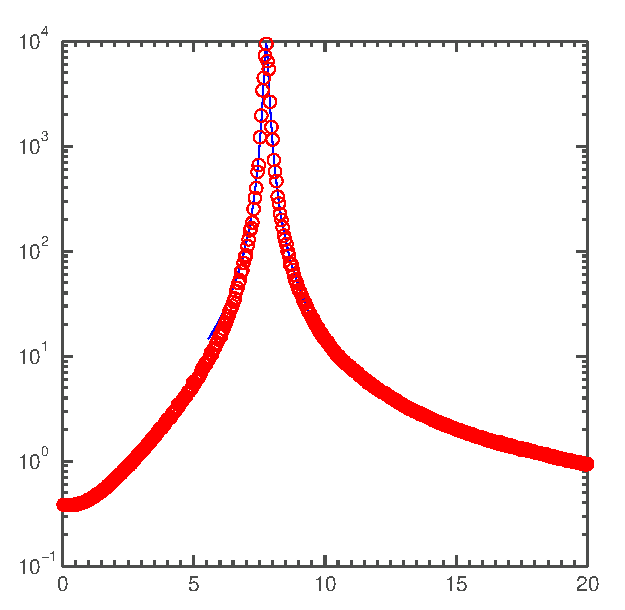
\includegraphics{sed.eps}}
\renewcommand{\figure}{Fig.}
\caption{(Colour online) Power spectra for selected modes of the $4\times 4$ [indicated by the labeled gray square markers in Figs.~\ref{fig:dispersion}(a-c)]. Dark blue corresponds to a superlattice without mixing, red corresponds to mixing of 80/20 and light blue corresponds to mixing of 60/40. Reported lifetimes calculated from the fitting of the Lorentzian functions (not shown) are identified by the subscripts.}
\label{fig:sed}
\end{center}
\end{figure*}
%%%

%The consequences of using same set of eigenvectors were used in the NMD procedure for mixed and non-mixed $N\times N$ is observed in Figure~\ref{fig:sed}, where for modes at low and high frequency, the peaks remain well-defined, but some intermediate frequency modes become noticeably perturbed.  
%%%
%\begin{figure}%[H]
%\begin{center}
%\scalebox{0.8}{ 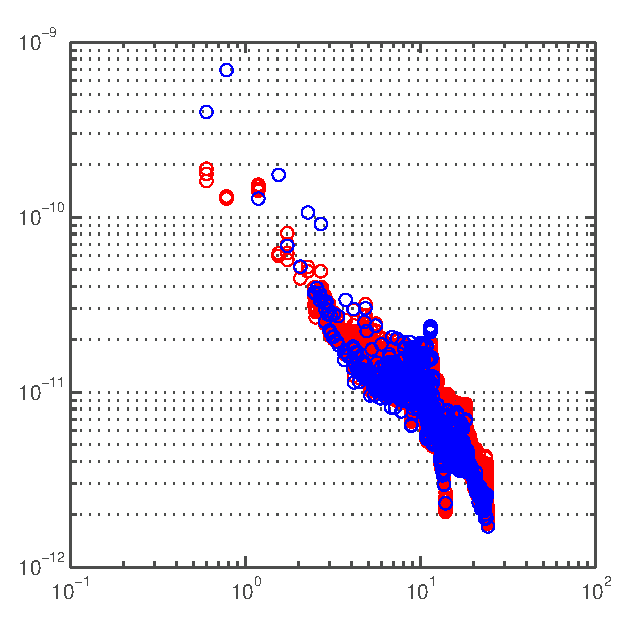
\includegraphics{/home/schuberm/Dropbox/git/plots.nogit/images/NMD_v_ALD.eps}}
%\renewcommand{\figure}{Fig.}
%\caption{Comparison between lifetimes from NMD and ALD in a $4\times4$ superlattice without interfacial mixing.}
%\label{FIG:NMD_v_ALD}
%\end{center}
%\end{figure}
%%%
%Confirm the validity of ALD

%Figure~\ref{FIG:NMD_v_ALD} shows no systematic bias between ALD and NMD for shorter lifetimes, with some systematic scatter at the longer lifetimes towards ALD. In general, ALD lifetimes are expected to be larger than NMD lifetimes because ALD neglects the contribution from $n$ order phonon processes\cite{PhysRevB.79.064301,esfarjani2011heat}, where $n$ is greater than 3.

\subsection{Lifetimes}

The phonon lifetimes as a function of $\omega_H \kv$ are plotted in Fig.~\ref{FIG:lifetime}. The lifetimes for all superlattices exhibit $\omega^{-2}$ scaling at low frequencies, consistent with theoretical predictions for modes in the Debye regime associated with quadratic behaviour found in the density of states at these frequencies as seen in Fig.~\ref{fig:dispersion}(d).\cite{Klemens_Thermal_1951} As the period length increases, the minimum frequency decreases and thus longest lifetime increases. This is a consequence of the increasing the number of atoms in the unit cell while conserving the number of unit cells used in the simulation. For $4\times4$, $8\times8$ and $14\times14$ superlattices, the perfect systems have two distinct trends that terminate at the maximum frequencies of the corresponding bulk systems (vertical lines in Fig.~\ref{FIG:lifetime}). The magnitudes of the lifetimes do not vary significantly across perfect superlattices and are comparable to the corresponding frequencies found in bulk.

Rayleigh scattering scaling, $\tau \propto \omega^{-4}$, was theoretically predicted under the Debye approximation, to predominantly affect lower-frequency modes due to elastic defect scattering.\cite{PhysRev.140.A1812,klemens_scattering_1955-3, klemens_thermal_1957-2}
As interspecies mixing is introduced to the superlattices the $\omega^{-4}$ scaling is observed at intermediate frequencies for $2\times2$ and $4\times4$ superlattices but not for $8\times8$ and $14\times14$ superlattices. The complicated dispersions of the superlattices, particularly for the $8\times8$ and $14\times14$ cases where there is a significant amount of branch folding, are not Debye-like at the intermediate frequencies such that the lifetimes diverge from the $\omega^{-4}$ scaling. The lifetimes of low frequency modes for all superlattices are not affected by the mixing and follow a similar $\omega^{-2}$ scaling as seen in the perfect superlattices.
%Because the $\tau\kv$ defined by the spectral width in Eq.(\ref{EQ:lifetime}) corresponds to all possibles mechanisms of phonon interaction, the $\omega^{-4}$ scaling diverges at low frequencies and is replaced by a $\omega^{-2}$ scaling. 

Mixing broadens the power spectra (Fig.~\ref{fig:sed}) and shifts the phonon lifetimes downward (Fig.~\ref{FIG:lifetime}), particularly for the intermediate and higher frequency modes. For $2 \times 2$ and $ 4 \times 4$ superlattices,  the lifetimes of some higher frequency modes fall below the Ioffe-Regel limit, $\tau =2\pi/\omega$, the limit where a mode has a lifetime equal to its period of oscillation. The normal modes for a perfect superlattice have a plane wave structure. Under the assumption that the normal modes of a perfect superlattice are representative of a mixed superlattice, reaching the Ioffe-Regel limit is therefore not an indication of spatial localization but rather of temporal localization. Modes that are below this limit can thus be considered to be non-propagating delocalized modes (diffusons).\cite{allen_thermal_1993,allen1999diffusons} Similar trends in the variation of lifetimes with frequency, dropping below the Ioffe-Regel limit at intermediate frequencies and then rising above at higher frequencies, have also been predicted for LJ alloys.\cite{jason2013vc} Spatial localization has previously been invoked to explain the period-length dependence of superlattice thermal conductivity, \cite{PhysRevB.61.3091} but this mechanism is not applicable to the systems studied here.

%%%
\renewcommand{\textfraction}{0.0}
\begin{figure}%[H]
\begin{center}
%\scalebox{1}{ \includegraphics{/Users/mullspace/Dropbox/git/plots.nogit/images/lifvomega.eps}}
\scalebox{1}{ \includegraphics{lifvomega.eps}}
\renewcommand{\figure}{Fig.}
\caption{Lifetimes for perfect (blue) and 80/20 (red) superlattices. The black line corresponds to the Ioffe-Regel criterion, $2\pi\omega^{-1}$. The brown line corresponds to $\omega^{-2}$ scaling. The green line corresponds to $\omega^{-4}$ scaling. Vertical grey lines correspond to the maximum frequency observed in the bulk systems: for the lighter species, $\omega_{max}=24.7$ and for the heavier species, $\omega_{max}=14.3$. } 
\label{FIG:lifetime}
\end{center}
\end{figure}
%%%

%Fig.~\ref{FIG:lifetime} shows general agreement between the lifetimes calculated using Eq.~(\ref{EQ:tau_eff}) and lifetimes obtained from NMD under the assumption that the eigenvectors of the unmixed systems are valid for the mixed systems; both resolve the $\omega^{-2}$ scaling at low frequencies and the general smearing at intermediate and larger frequencies. At larger frequencies, Tamura theory predicts lifetimes below the Ioffe-Regel limit for all superlattice period lengths.
%%%
\begin{comment}
\begin{table}
\begin{center}
\begin{tabular*}{\textwidth}{c@{\extracolsep{\fill}}ccccc}
\hline\hline\noalign{\smallskip}
&\multicolumn{3}{c}{$N\times N$ Superlattice} \\
\cline{2-5}\noalign{\smallskip}
\hspace{1cm} & $2\times2$ & $4\times4$ & $8\times8$ & $14\times14$  \\
\noalign{\smallskip}\hline\noalign{\smallskip}
%$\tau_{eff}$   & 0.51 $\pm$ 0.51 & 0.49 $\pm$ 0.59 &  0.33 $\pm$ 0.34& 0.21 $\pm$ 0.22 \\
%ALD   & 0 $\pm$ 0 & 0.11  $\pm$  0.14 &  0.09  $\pm$  0.07 & NA \\
RMSE $\sqrt{\frac{\sum_{\pmb{\kappa}\nu}(\tau_{eff}\kv-\tau_{mixed}\kv)^2}{n}}$ &0.65 & 1.21 & 2.09 & 5.42\\
Mean $\overline{\tau_{mixed}\kv}$ &1.37 & 1.93 & 2.74 & 3.40\\
Standard Deviation $\sigma[\tau_{mixed}\kv]$ &2.34 & 2.66 & 5.53 & 11.84\\
\noalign{\smallskip}\hline\hline
\end{tabular*}
\end{center}
\renewcommand{\table}{Table.}
\caption{The root-mean-square error between Tamura theory effective lifetimes and NMD mixed lifetimes. The mean and standard deviation of the NMD mixed lifetimes are provided for context. %ALD was not used for the 14x14 case due to the computational complexity of $\Omega (N_{uc}^4)$.}
}
\label{TB:taud}
\end{table}
\end{comment}
%%%

\subsection{Thermal Conductivity}

\begin{table*}
\begin{center}
\begin{tabular*}{\textwidth}{c@{\extracolsep{\fill}}cccccc}
\hline\hline\noalign{\smallskip}
\multicolumn{2}{c}{\multirow{2}{*}{Cross-Plane}}& \multicolumn{4}{c}{$N\times N$ Superlattice} \\
\cline{3-6}\noalign{\smallskip}
\hspace{1cm} && $2\times2$ & $4\times4$ & $8\times8$ & $14\times14$  \\
\noalign{\smallskip}\hline\noalign{\smallskip}
\multirow{3}{*}{Perfect} &NMD & 0.29 $\pm$ 0.03 & 0.23 $\pm$ 0.02 & 0.32 $\pm$ 0.03 & 0.39 $\pm$ 0.04 \\
&GK & 0.25 $\pm$ 0.02 & 0.22 $\pm$ 0.02  &  0.29 $\pm$ 0.02  &  0.39 $\pm$ 0.03\\
%&ALD & 0.25 &	0.26  &	0.32	 &0.44\\
&Thermal Circuit & 0.07  &  0.13  &  0.23  &  0.32\\
\noalign{\smallskip}\hline
\multirow{3}{*}{Mixed} &NMD &0.19 $\pm$ 0.02& 0.17 $\pm$ 0.02& 0.28 $\pm$ 0.03 & 0.42$\pm$ 0.04\\
&GK  & 0.16 $\pm$ 0.01  &  0.18 $\pm$ 0.02 &  0.29 $\pm$ 0.02 &   0.45 $\pm$ 0.06\\
&Tamura (NMD) & 0.21 $\pm$ 0.02& 0.15 $\pm$ 0.02& 0.30 $\pm$ 0.03& 0.37$\pm$ 0.04\\
%&Tamura (ALD) & 0.12 & 0.19 & 0.26 & 0.40\\
\hline\hline
\end{tabular*}
\end{center}
\renewcommand{\table}{Table.}
\caption{A comparison of the cross-plane thermal conductivity predictions [W/m K].}
\label{TB:K_CP}
\end{table*}

\begin{table*}
\begin{center}
\begin{tabular*}{\textwidth}{c@{\extracolsep{\fill}}cccccc}
\hline\hline\noalign{\smallskip}
\multicolumn{2}{c}{\multirow{2}{*}{In-Plane}}&\multicolumn{4}{c}{$N\times N$ Superlattice} \\
\cline{3-6}\noalign{\smallskip}
\hspace{1cm} && $2\times2$ & $4\times4$ & $8\times8$ & $14\times14$  \\
\noalign{\smallskip}\hline\noalign{\smallskip}
\multirow{2}{*}{Perfect} &NMD &0.52$\pm$ 0.05 & 0.51 $\pm$ 0.05& 0.56 $\pm$ 0.05& 0.60$\pm$ 0.06\\
&GK &0.53 $\pm$ 0.03 &  0.54 $\pm$ 0.03 &  0.61 $\pm$ 0.05  &  0.66 $\pm$ 0.07 \\
%&ALD & 0.55	& 0.53	&	0.59 	&0.63\\
\noalign{\smallskip}\hline
\multirow{3}{*}{Mixed} & NMD &0.21 $\pm$ 0.02 & 0.25 $\pm$ 0.03 & 0.37 $\pm$ 0.04 & 0.47  $\pm$ 0.05\\
&GK & 0.19 $\pm$ 0.02 &  0.30 $\pm$ 0.01  & 0.43$\pm$ 0.03 &  0.62 $\pm$ 0.07 \\   
&Tamura (NMD)& 0.22 $\pm$ 0.02 & 0.27 $\pm$ 0.03 & 0.38 $\pm$ 0.04 & 0.45 $\pm$ 0.05\\
%&Tamura (ALD) & 0.17 & 0.25 & 0.34 &0.38\\
\hline\hline
\end{tabular*}
\end{center}
\renewcommand{\table}{Table.}
\caption{A comparison of the in-plane thermal conductivity predictions [W/m K].}
\label{TB:K_IP}
\end{table*}
%%%
\subsubsection{Perfect superlattices}
With reference to Tables~\ref{TB:K_CP} and~\ref{TB:K_IP}, the trends in cross-plane and in-plane thermal conductivity predictions from NMD and GK for perfect superlattices are in good agreement. In-plane thermal conductivity increases with increasing period length, while cross-plane thermal conductivity first decreases then increases with period length consistent with previous MD superlattice studies. \cite {PhysRevB.72.174302} In-plane thermal conductivity is nearly a factor of two larger than cross-plane thermal conductivity for all superlattices. A thermal circuit model is presented in Table~\ref{TB:K_CP}. The boundary resistance for a perfect interface, estimated from the Direct Method ($R_{int}=1.4065\times10^{-8}$ Km$^2$W$^{-1}$), was combined with bulk thermal conductivities of the lighter material ($k_{m}$=1.2 W/mK) and the heavier material ($k_{3m}$=0.7 W/mK) through their respective layer thickness, yielding an effective resistance that was inverted to obtain an effective thermal conductivity 
%%%
\begin{equation}\label{EQ:TCircuit}
\begin{split}
k_{circuit}= \frac{La}{R_{int}+\frac{La}{2k_m}+\frac{La}{2k_{3m}}}.
\end{split}
\end{equation}
The thermal circuit model underestimates the thermal conductivity for all superlattices, with the relative difference decreasing with increasing period length, an indication that the this model may become representative of the nature of thermal transport at large enough period lengths.
%%%
%No minimum in cross-plane thermal conductivity is found in the ALD predictions.
\subsubsection{Mixed superlattices}
To provide insight into the assumption of using the perfect superlattice eigenvectors for the mixed superlattices, we use Tamura elastic mass-defect scattering theory \cite{tamura_isotope_1983} to modify the lifetimes predicted for perfect superlattices, $\tau_{perfect}\kv$, through the Matthiesen rule as done by Luckyanova et al. \cite{Luckyanova16112012} 
%%%
\begin{equation}\label{EQ:tau_eff}
\begin{split}
\frac{1}{\tau_{effective}\kv} = \frac{1}{\tau_{defect}\kv}+\frac{1}{\tau_{perfect}\kv} ,
\end{split}
\end{equation}
%%%
where
%%%
\begin{equation}\label{EQ:tau_d}
\begin{split}
\frac{1}{\tau_{defect}\kv} = &\frac{\pi}{2N_{uc}}\omega^2\kv \sum_{\pmb{\kappa'},\nu'} \delta\left[ \omega\kv - \omega\kvp \right]\\
&\sum_{b} g_2(b) |e^*\kvbap \cdot e\kvba |^2 .
\end{split}
\end{equation}
%%%
Here, $N_{uc}$ is the total number of unit cells considered, and $g_2(b)$ is the coupling term for atom $b$ in the unit cell that defines the strength of the mass disordering
%%%
\begin{equation}\label{EQ:g(b)}
\begin{split}
g_2(b) = \sum_\mu c_{\mu}(b)\left[1-\frac{m_{\mu}(b)}{\overline{m(b)}}\right]^2, 
\end{split}
\end{equation}
%%%
where the summation is over the possible species at that atomic position in the unit cell with the concentration $c_\mu(b)$, mass $m_\mu(b)$ and average mass $\overline{m(b)}$. Given that there are two atom types in the superlattice unit cell, the lighter atom can be considered to be a mass defect of the heavier portion of the superlattice, and vice-versa. $g_2(b)$ is zero if atom $b$ was unmixed (i.e., for atoms that do not reside within one monolayer of the interface). The delta function in Eq.~(\ref{EQ:tau_d}) is broadened into a Lorentzian function with width on the order of the frequency level spacing (i.e.: min[$\omega_i \kv -\omega_j \kv$]) imposed by the finite size of the systems.\cite{allen_thermal_1993}

For short period mixed superlattices, the in-plane and cross-plane predictions are reduced from their corresponding perfect system and approach the alloy limit (0.21 W/mK from GK using $N_{x,y,z}=6$), with the mixed $2\times 2$ losing much of its anisotropy between the in-plane and cross-plane directions. From Table~\ref{TB:K_CP}, the predictions for mixed superlattices from NMD (using perfect eigenvectors), Tamura theory and GK follow similar trends, with increasing cross-plane thermal conductivity with increasing period length. From Table~\ref{TB:K_IP}, for mixed superlattices with the exception of $2 \times 2$, NMD and Tamura theory, while in good agreement respectively,  predict a lower in-plane thermal conductivity, with the systematic difference increasing with period length. This is indicative of the disruption of the superlattice phonon modes through interfacial mixing which are expected to contribute to thermal transport. 
%With increasing period length, these modified modes are more likely to be represented by bulk-like modes and may explain the discrepancy between NMD or Tamura theory and GK.
%The successful application of Tamura's elastic defect scattering theory to systems studied here is consistent with Pomeranchuk's argument that inelastic defect scattering has negligible effects upon thermal transport.\cite{pomeranchuk1942thermal} 
%%%
\begin{comment}
\begin{table}
\begin{center}
\begin{tabular}{lcc}
\hline\hline\noalign{\smallskip}
&\multicolumn{2}{c}{Method} \\
\cline{2-3}\noalign{\smallskip}
$k$ & NMD  & GK  \\
\noalign{\smallskip}\hline\noalign{\smallskip}
Cross-Plane Perfect  & 0.24 $\pm$ 0.02 & 0.22 $\pm$ 0.04\\
Cross-Plane 80/20    & 0.17  $\pm$ 0.01   &   0.18 $\pm$ 0.02 \\
Cross-Plane 60/40    & 0.18  $\pm$ 0.01   &   0.19 $\pm$ 0.02 \\
In-Plane Perfect   & 0.52 $\pm$ 0.03 & 0.54 $\pm$ 0.03  \\
In-Plane 80/20  & 0.25 $\pm$ 0.02 & 0.30 $\pm$ 0.01  \\
In-Plane 60/40   & 0.20 $\pm$ 0.02 & 0.26 $\pm$ 0.01  \\
\noalign{\smallskip}\hline\hline
\end{tabular}
\end{center}
\renewcommand{\table}{Table.}
\caption{A comparison of the thermal conductivity predictions [$Wm^{-1}K^{-1}$] predictions for a $4\times4$ superlattice.}
\label{TB:validate}
\end{table}
\end{comment}
%%%
\begin{comment}
\subsubsection{MFP spectrum}
The plots of the CP thermal conductivity MFP contribution curves, defined by
%%%
\begin{equation}\label{EQ:MFP_contr}
\begin{split}
dk(\lambda)=\lambda\kv d\lambda, 
\end{split}
\end{equation}
%%%
is shown in Fig.~\ref{FIG:MFP_cp}. There is a clear reduction in the contribution to cross-plane thermal conductivity in perfect superlattices from modes with a MFP greater than the period length as period length increases. This trend is consistent with the theoretical predictions from Mahan that a minimum thermal conductivity occurs as the transport behaviour shifts from a wave-regime to particle-regime.\cite{PhysRevLett.84.927,PhysRevB.56.10754} This same trend is observed in the contribution curves for the in-plane conductivity (not shown). The minimum cross-plane thermal conductivity in the for perfect superlattices occurs at a point where the average MFP is slightly greater than the period length ($4 \times 4$). The dimensional value of the peak MFP in perfect superlattices, for both in-plane and cross-plane, does not vary significantly as a function of period length. 

For short period superlattices ($2\times2$, $4\times4$ and $8\times8$), interfacial mixing shifts the average MFP towards the period length and reduces its respective contribution, indicative of the transition of thermal transport from superlattice phonons to thermal transport from phonons which may or may not map to those belonging to the perfect dispersion. This trend further supports the fact that superlattice phonons become disrupted by interfacial mixing, thereby diminishing the enhancing effects of the secondary periodicity upon cross-plane thermal conductivity. At large enough period lengths, the effect of interspecies mixing has a negligible effect on phonon MFP, as the corresponding lifetimes are less affected with increasing period length (Fig.~\ref{FIG:lifetime}) because of the decrease in the number of interfaces per unit of volume. \cite{PhysRevB.79.075316}
%%%
\begin{figure}%[H]
\begin{center}
\scalebox{1}{ \includegraphics{MFP_cp.eps}}
\renewcommand{\figure}{Fig.}
\caption{Phonon mean free path normalized by the period length contribution to the cross-plane thermal conductivity. From top to bottom $2\times2$, $4\times4$, $8\times8$ and $14\times14$ superlattices. Color corresponds to those used in Fig.~\ref{FIG:lifetime}. Average MFP is reported; subscripts correspond to the color of marker [b:blue (perfect), r:red (mixed)]. Orange corresponds to lighter bulk and green corresponds to heavier bulk.}
\label{FIG:MFP_cp}
\end{center}
\end{figure}
%%%

The noise in the contribution distribution at longer MFPs is consequence of the limited resolution of the Brouillin zone enforced by the MD domain. This has been observed in other mode by mode analysis techniques, such as the real space force constant extraction from DFT method used by Esfarjani, where the limited resolution manifested in a stepwise behavior of thermal conductivity accumulation function of bulk silicon. \cite{PhysRevB.84.085204} The linear behavior of the dispersion near the gamma point of the Brouillin zone and the $\omega^{-2}$ scaling of the lifetimes allowed for the contribution of these unresolved long-wavelength modes to be estimated. The linear extrapolation procedure used to predict bulk thermal conductivities \cite{PhysRevB.81.214305} was not used in previous superlattice studies \cite{doi:10.1021/nl202186y,Luckyanova16112012} and is not used here. The complicated dispersion [Fig.~\ref{fig:dispersion}(a-c)] does not guarantee that such an approach is viable, as such, understanding size effects in superlattices warrants further work.
\end{comment}

\section{Superlattice phonons}\label{SEC:sl_phon}

The term ``coherence" has been used in two distinct contexts in relation to phonons. First, coherence is used to describe the constructive or destructive interference from the phase preserving reflection of phonons off a secondary periodicity (i.e.: superlattices or a silicon thin films with periodic arrangement of holes\cite{doi:10.1021/nl102918q}). The second context is used to describe the excitation of long wavelength phonons, usually by femtosecond time-resolved pump-probe techniques \cite{PhysRevLett.73.740,PhysRevB.75.195309}, that do not carry much thermal energy and are not found in the MD simulations studied here. While both contexts imply the wave picture of vibrational modes, the former context and its relation to thermal transport is the focus of this section.

In solids, the phonons that carry thermal energy belong to the dispersion relation of that material, which depends on the geometry, the harmonic force constants and constituent masses. Thus the introduction of a secondary periodicity can modify the dispersion such that the modes which emerge do not exist in the composing bulk materials. These non-bulk phonons (in this case, superlattice phonons) propagate and scatter in the periodic structure in a similar manner to what a bulk phonon undergoes in a bulk material. Do these superlattice phonons experience the first context of coherence; in other words, does a superlattices phonon reflect off a superlattice's interface and interfere with another superlattice phonon?%Coherent effects, for that matter, are found in bulk systems since coherence requires the constructive or destructive interference of waves.

%of vibrational modes when a secondary periodicity is added to a system (i.e.: superlattices or a silicon thing file with periodic arrangement of holes),
%The reasons are twofold for the ambiguity attached to the terms \textit {coherent phonon}: its association with exotic configurations of material, like porous silicon \cite{doi:10.1021/nl102918q} where the secondary periodicity emerges from the introduction of the repeated holes or between nanoparticles in a nanofluidic system \cite{Keblinski2002855} and from previous femtosecond time-resolved pump-probe experimental coherent phonon studies \cite{PhysRevLett.73.740,PhysRevB.75.195309} that do not focus upon thermal transport. Coherent effects, for that matter, are found in bulk systems since coherence requires the constructive or destructive interference of waves.

Past literature has cited the superlattice as a structure where coherent effects on thermal transport are possible; the trend in cross-plane thermal conductivity as a function of period length being used to justify such a claim. \cite{PhysRevB.67.195311,PhysRevB.72.174302,PhysRevB.61.3091} and it is theorized that the minimum corresponds to the transition from wave-governed transport to particle-governed transport.\cite{PhysRevLett.84.927,PhysRevB.56.10754} Here, we have observed a minimum in perfect superlattices simply by adopting the correct phonon dispersion for our analysis. By using MD simulations, we do not impose any restrictions on the phonon dynamics but let the system move through phase space naturally and thus should sufficiently capture all classical effects, including coherent effects. The results presented in this work suggest that using the correct normal modes is sufficient to capture the physics of thermal transport in a perfect superlattice, implying a dispersion effect. Dispersion effects are of consequence when one cannot use the bulk material phonon properties as particles to predict thermal transport in a non-bulk system. This is clearly the case for all the systems studied here (perfect and mixed), including the larger period superlattices ($8 \times 8$ and $14 \times 14$), as evidenced by the discrepancy between the bulk-based thermal circuit model predictions and the NMD and GK predictions (see Table~\ref{TB:K_CP}).

Coherence length, defined as the distance a plane wave travels until its phase becomes randomized, only applies to the wave picture of phonon transport. Although there does not appear to be a formal equation for phonon coherence length,\cite{chen2005nanoscale} adopting a unit cell that spans a single superlattice period to generate the modified dispersion relation allows one to ignore the difference between the MFP and coherence length\cite{PhysRevB.67.195311} because the phonons are not localized to a single layer (as confirmed by the participation ratio) and in the perfect superlattice case, the only inelastic scattering mechanism (phase randomizing) is the anharmonicity of the LJ potential. The plots of the CP thermal conductivity MFP contribution curves, defined by
%%%
\begin{equation}\label{EQ:MFP_contr}
\begin{split}
dk_{\alpha}(\Lambda \kv)=c_{ph}\kv v^2_{g,\alpha}\kv \frac{\Lambda \kv} {|\pmb{\mathrm{v}}_{g}\kv|} d\Lambda \kv, 
\end{split}
\end{equation}
%%%
is shown in Fig.~\ref{FIG:MFP_cp}. 
%%%
\begin{figure}%[H]
\begin{center}
\scalebox{1}{ \includegraphics{MFP_cp.eps}}
\renewcommand{\figure}{Fig.}
\caption{Phonon mean free path normalized by the period length contribution to the cross-plane thermal conductivity. Color corresponds to those used in Fig.~\ref{FIG:lifetime}. Average MFP is reported. Orange corresponds to lighter bulk and green corresponds to heavier bulk.}
\label{FIG:MFP_cp}
\end{center}
\end{figure}
%%%
There is a clear reduction in the contribution to cross-plane thermal conductivity in perfect superlattices from modes with a MFP greater than the period length as period length increases. This trend is consistent with the theoretical predictions from Mahan that a minimum thermal conductivity occurs as the transport behaviour shifts from a wave-regime to particle-regime when the average MFP transitions from being greater than the period length to being less than the period length.\cite{PhysRevLett.84.927,PhysRevB.56.10754} This same trend is observed in the contribution curves for the in-plane conductivity (not shown). The minimum cross-plane thermal conductivity for perfect superlattices occurs at a point where the average MFP is greater than the period length ($4 \times 4$), as described by Mahan.\cite{PhysRevLett.84.927} In the perfect superlattice case, the MFPs greater than the period length cannot be interpreted any differently than MFPs greater than the lattice constant of a bulk crystalline structure (in other words, the MFPs greater than the superlattice period length do not manifest because of phase-preserving reflection from the interfaces). This statement is confirmed by observing that MFP contribution distribution, normalized by the superlattice period length, for the lighter (orange) and heavier (green) bulk systems (Fig.~\ref{FIG:MFP_cp}) follows the MFP distribution for the perfect superlattices. We do not find evidence that superlattice phonons experience coherent effects and believe that thermal transport in perfect superlattices is accurately represented by the corresponding dispersion relation.%The dimensional value of the peak MFP in perfect superlattices, for both in-plane and cross-plane, does not vary significantly as a function of period length.

For short period superlattices ($2\times2$, $4\times4$ and $8\times8$), interfacial mixing shifts the average MFP towards the period length and reduces its respective contribution, indicative of the transition of thermal transport from superlattice phonons to thermal transport from phonons which may or may not map to those belonging to the perfect dispersion. %This trend further supports the fact that superlattice phonons become disrupted by interfacial mixing, thereby diminishing the enhancing effects of the secondary periodicity upon cross-plane thermal conductivity. 
The assumption of the validity of perfect superlattice eigenvectors captures the downward shift in the MFP distributions and generates a discrepancy between GK and Tamura theory or NMD predictions for in-plane thermal conductivity. These results suggest that roughness and disorder disrupt the dispersion effect. At large enough period lengths ($14\times14$), the effect of interspecies mixing has a negligible effect on phonon MFP, as the corresponding lifetimes are less affected with increasing period length (Fig.~\ref{FIG:lifetime}) because of the decrease in the number of interfaces per unit of volume. \cite{PhysRevB.79.075316}

%Mixing introduces an additional scattering mechanism, modeled in Tamura theory as an elastic mass defect. Elastic scattering implies that the wavevector of the incident phonon does not undergo a change in magnitude but only experiences a change in direction and thus is a phase preserving event. However, the use of the Matthiesen rule effectively masks any distinction between anharmonic scattering and defect scattering by encapsulating the overall effect as inelastic scattering. The assumption of the validity of perfect superlattice eigenvectors captures the downward shift in the MFP distributions but generates a discrepancy between GK and Tamura theory or NMD predictions for in-plane thermal conductivity. These results suggest that roughness and disorder disrupt the dispersion effect.% and non-superlattice phonons, but not necessarily bulk-like phonons, may be more representative.%, consequently destroying coherent effects (inelastic scattering may be more representative).\cite{PhysRevB.67.195311,dames_682} 

%Phase is assumed to be randomized through inelastic phonon-phonon, but not elastic boundary or impurity scattering \cite{chen2005nanoscale}. Furthermore, the inability for NMD and ALD to estimate the in-plane thermal conductivity in mixed superlattices indicates the disruption of the superlattice dispersion. 

%Finally, by relying upon the BTE, any coherent effect is abstracted into the phonon-as-a-particle interpretation.
\section{Summary}

We show the reduction in the contribution to cross-plane thermal conductivity from MFPs greater than the superlattice period as the period length is increased, for both perfect and mixed superlattices. Differences between in-plane and cross-plane components of group velocity are responsible for the respective differences between thermal conductivity [Fig.~\ref{fig:dispersion}(a-c)]. Debye scaling at low frequency modes in perfect and mixed superlattices and Raleigh scattering at intermediate frequencies in mixed superlattices is observed (Fig.~\ref{FIG:lifetime}). Interspecies mixing reduces phonon lifetimes thereby shifting the phonon MFP spectrum downward (Fig.~\ref{FIG:MFP_cp}) and disrupts superlattice phonon transport (Fig.~\ref{fig:sed}(B) and Table~\ref{TB:K_IP}), thus reducing in-plane and cross-plane thermal conductivity.

\section{Acknowledgements}
SCH and CHA acknowledges the support of OGS, NSERC and AMD. JML and AJHM acknowledge the support from AFOSR award FA95501010098. Simon Lu performed the Direct Method simulations.

\newpage
\section{Appendix: Size effects}
Mode-by-mode studies are computationally expensive and accounting for size effects is challenging. Broido et al. were limited to a range of short period lengths ($8\times 8$) for Si/Ge.\cite {PhysRevB.70.081310} For similar reasons, the phonon properties for short period Si/Ge superlattices obtained from DFPT were presumed to hold for larger period superlattices \cite{Luckyanova16112012, doi:10.1021/nl202186y} and the phonon lifetimes of low frequency modes used in the Monte Carlo BTE approach are fitted to a power law. \cite{savic:073113} 

A comparison of the thermal conductivity predictions is presented in Tables~\ref{TB:K_CP_NMDsize} (cross-plane) and~\ref{TB:K_IP_NMDsize} (in-plane). The NMD predictions for both the cross-plane and in-plane thermal conductivities varied by about 10\% when increasing $N_x=6$ to $N_x=8$ along the cross-plane and fixing $N_y=N_z=6$ unit cells along the in-plane ($N_x=10$ was used for the $2\times2$ superlattices to resolve the lifetime scalings). Unlike the previous mode-by mode studies, the phonon properties of short period superlattices was not extended to large period superlattices. Due to the time complexity of the NMD algorithm [$O(12N_xN_yN_z L)$], however, further increasing the Brouillin zone resolution ($N_i$) was computationally prohibitive. As a result of these size effects, the reported thermal conductivity predictions from NMD are presumed to carry an uncertainty of 10\%. Uncertainty in the GK prediction was found by systematically removing one seed before specifying the thermal conductivity.

One approach to estimating size effects is to conduct simulations for a range of system sizes, linearly extrapolate the inverse thermal conductivity with respect to the inverse length of the system and take the y-intercept as the bulk value.\cite{PhysRevB.81.214305}  % where the linear behavior of the dispersion near the gamma point of the Brouillin zone and the $\omega^{-2}$ scaling of the lifetimes allowed for the contribution of these unresolved long-wavelength modes to be estimated. \cite{PhysRevB.81.214305} 
This method was not used in the previous superlattice studies \cite{doi:10.1021/nl202186y,savic:073113,Luckyanova16112012} and is not used here. The complicated dispersion [Fig.~\ref{fig:dispersion}(a-c)] does not guarantee that such an approach is viable, as such, understanding size effects in superlattices warrants further work.

\begin{table*}
\begin{center}
\begin{tabular*}{\textwidth}{c@{\extracolsep{\fill}}ccccc}
\hline\hline\noalign{\smallskip}
Cross-Plane Perfect& \multicolumn{4}{c}{Superlattice} \\
\cline{2-5}\noalign{\smallskip}
$N_x\times N_y \times N_z$ & $2\times2$ & $4\times4$ & $8\times8$ & $14\times14$  \\
\noalign{\smallskip}\hline\noalign{\smallskip}
$4\times6\times6$ & 0.15  & 0.17  &  0.15  &  0.21 \\
$6\times6\times6$ & 0.23  & 0.22  &  0.28  &  0.36 \\
$8\times6\times6$ & 0.28  & 0.23  &  0.32  &  0.39 \\
$10\times6\times6$ & 0.29  &  - &  -  &  - \\
\hline\hline
\end{tabular*}
\end{center}
\renewcommand{\table}{Table.}
\caption{Size-dependent cross-plane thermal conductivity NMD predictions [Wm$^{-1}$K$^{-1}$].}
\label{TB:K_CP_NMDsize}
\end{table*}

\begin{table*}
\begin{center}
\begin{tabular*}{\textwidth}{c@{\extracolsep{\fill}}ccccc}
\hline\hline\noalign{\smallskip}
In-Plane Perfect& \multicolumn{4}{c}{Superlattice} \\
\cline{2-5}\noalign{\smallskip}
$N_x\times N_y \times N_z$ & $2\times2$ & $4\times4$ & $8\times8$ & $14\times14$  \\
\noalign{\smallskip}\hline\noalign{\smallskip}
$4\times6\times6$ & 0.53 & 0.52  &  0.56  &  0.69 \\
$6\times6\times6$ & 0.53 & 0.51  &  0.56  &  0.59 \\
$8\times6\times6$ & 0.52 & 0.51  &  0.55  &  0.58 \\
$10\times6\times6$ & 0.52 & -  &  -  &  - \\
\hline\hline
\end{tabular*}
\end{center}
\renewcommand{\table}{Table.}
\caption{Size-dependent in-plane thermal conductivity NMD predictions [Wm$^{-1}$K$^{-1}$].}
\label{TB:K_IP_NMDsize}
\end{table*}

%Furthermore, the linear extrapolation procedure cannot be applied because as size was increased, thermal conductivity was found to decrease.

\begin{comment}
\begin{table*}
\begin{center}
\begin{tabular*}{\textwidth}{c@{\extracolsep{\fill}}ccccc}
\hline\hline\noalign{\smallskip}
Cross-Plane& \multicolumn{4}{c}{$N\times N$ Superlattice} \\
\cline{2-5}\noalign{\smallskip}
$N_xN_yN_z$ & $2\times2$ & $4\times4$ & $8\times8$ & $14\times14$  \\
\noalign{\smallskip}\hline\noalign{\smallskip}
$6\times6\times6$ & 0.15 $\pm$ 0.02 & 0.22 $\pm$ 0.02  & 0.21 $\pm$ 0.03 &  \\
$8\times6\times6$ & 0.25 $\pm$ 0.02 & 0.22 $\pm$ 0.04  &  0.29 $\pm$ 0.02  &  0.39 $\pm$ 0.03\\
$8\times8\times8$ & 0.15 $\pm$ 0.01 & 0.17 $\pm$ 0.01  & 0.22 $\pm$ 0.02  &   \\
$10\times10\times10$ & 0.18 $\pm$ 0.01 & &   &  \\
$12\times12\times12$ & 0.19 $\pm$ 0.02 & &   &  \\
$16\times12\times12$& 0.19 $\pm$ 0.01 & 0.19 $\pm$ 0.01 &  0.21 $\pm$ 0.04  &  \\
\hline\hline
\end{tabular*}
\end{center}
\renewcommand{\table}{Table.}
\caption{A comparison of the cross-plane thermal conductivity GK predictions [Wm$^{-1}$K$^{-1}$].}
\label{TB:K_CP_GKsize}
\end{table*}

\begin{table*}
\begin{center}
\begin{tabular*}{\textwidth}{c@{\extracolsep{\fill}}ccccc}
\hline\hline\noalign{\smallskip}
In-Plane&\multicolumn{4}{c}{$N\times N$ Superlattice} \\
\cline{2-5}\noalign{\smallskip}
\hspace{1cm} & $2\times2$ & $4\times4$ & $8\times8$ & $14\times14$  \\
\noalign{\smallskip}\hline\noalign{\smallskip}
$8\times6\times6$ & 0.53 $\pm$ 0.03 &  0.54 $\pm$ 0.03 &  0.61 $\pm$ 0.05  &  0.66 $\pm$ 0.07 \\
$8\times8\times8$ & &   &    &  \\
$10\times10\times10$ &  &  &    &  \\
$12\times12\times12$ &  &   &    &  \\
$16\times12\times12$ & 0.53 $\pm$ 0.03 &  0.54 $\pm$ 0.04 &  0.62 $\pm$ 0.02  & \\
\hline\hline
\end{tabular*}
\end{center}
\renewcommand{\table}{Table.}
\caption{A comparison of the in-plane thermal conductivity GK predictions [Wm$^{-1}$K$^{-1}$].}
\label{TB:K_IP_GKsize}
\end{table*}
\end{comment}

\newpage
\bibliographystyle{apsrev}
\bibliography{superlattice.bib}

\end{document}

